
\section{Modeling in Ptolemy}
\label{sec:modeling-ptolemy}

In this section, we present the strategy we followed to implement in Ptolemy the MAC layer of OpenWSN\footnote{Though the model in each figure is vector graphics, and it is possible to zoom in and read all the details, we  suggest the reader to open the attached Ptolemy model for further information}.

In Figure~\ref{fig:OpenWSNNode}, on the left, a network of OpenWSN nodes is shown. We leveraged the Ptolemy multiform time to model clock drifts typical of real nodes. 

In this work, our focus has been the modeling of the TSCH state machine. However, to obtain a runnable model we have also modeled a simple physical-level radio and abstracted the higher network layers as a single application layer. Figure~\ref{fig:OpenWSNNode}, on the right, shows our stack of actors. We can see how the information flow proceed from the physical channel to the application layer and \emph{vice versa}. 

Taking a closer look, we defined each actor as follows:

{\bf PhysicalLayer:} This actor provides the interface to and from the physical channel and the rest of the network. Ports \texttt{fromPhysical}, \texttt{toPhysical}, \texttt{fromMAC} and \texttt{toMAC} are used to exchange data during both transmission and reception.
To simulate a realistic behavior, in which a packet needs a certain time to be received/sent, the \texttt{PhysicalLayer} actor adds delays whenever a packet needs to be forwarded in any direction. Ports \texttt{startOfFrame} and \texttt{endOfFrame} indicate to the MAC layer the beginning and the ending of a transmission/reception performed by the radio. 

{\bf AppLayer:} This actor represents the high level application running in each node. From a general point of view, the definition of the node global behavior is this actor's responsibility. It communicates with the MAC layer through ports \texttt{fromMAC} and \texttt{toMAC}. In this work we haven't implemented complex application models, leaving this task as a future work. 

\begin{figure}[t]
\centering
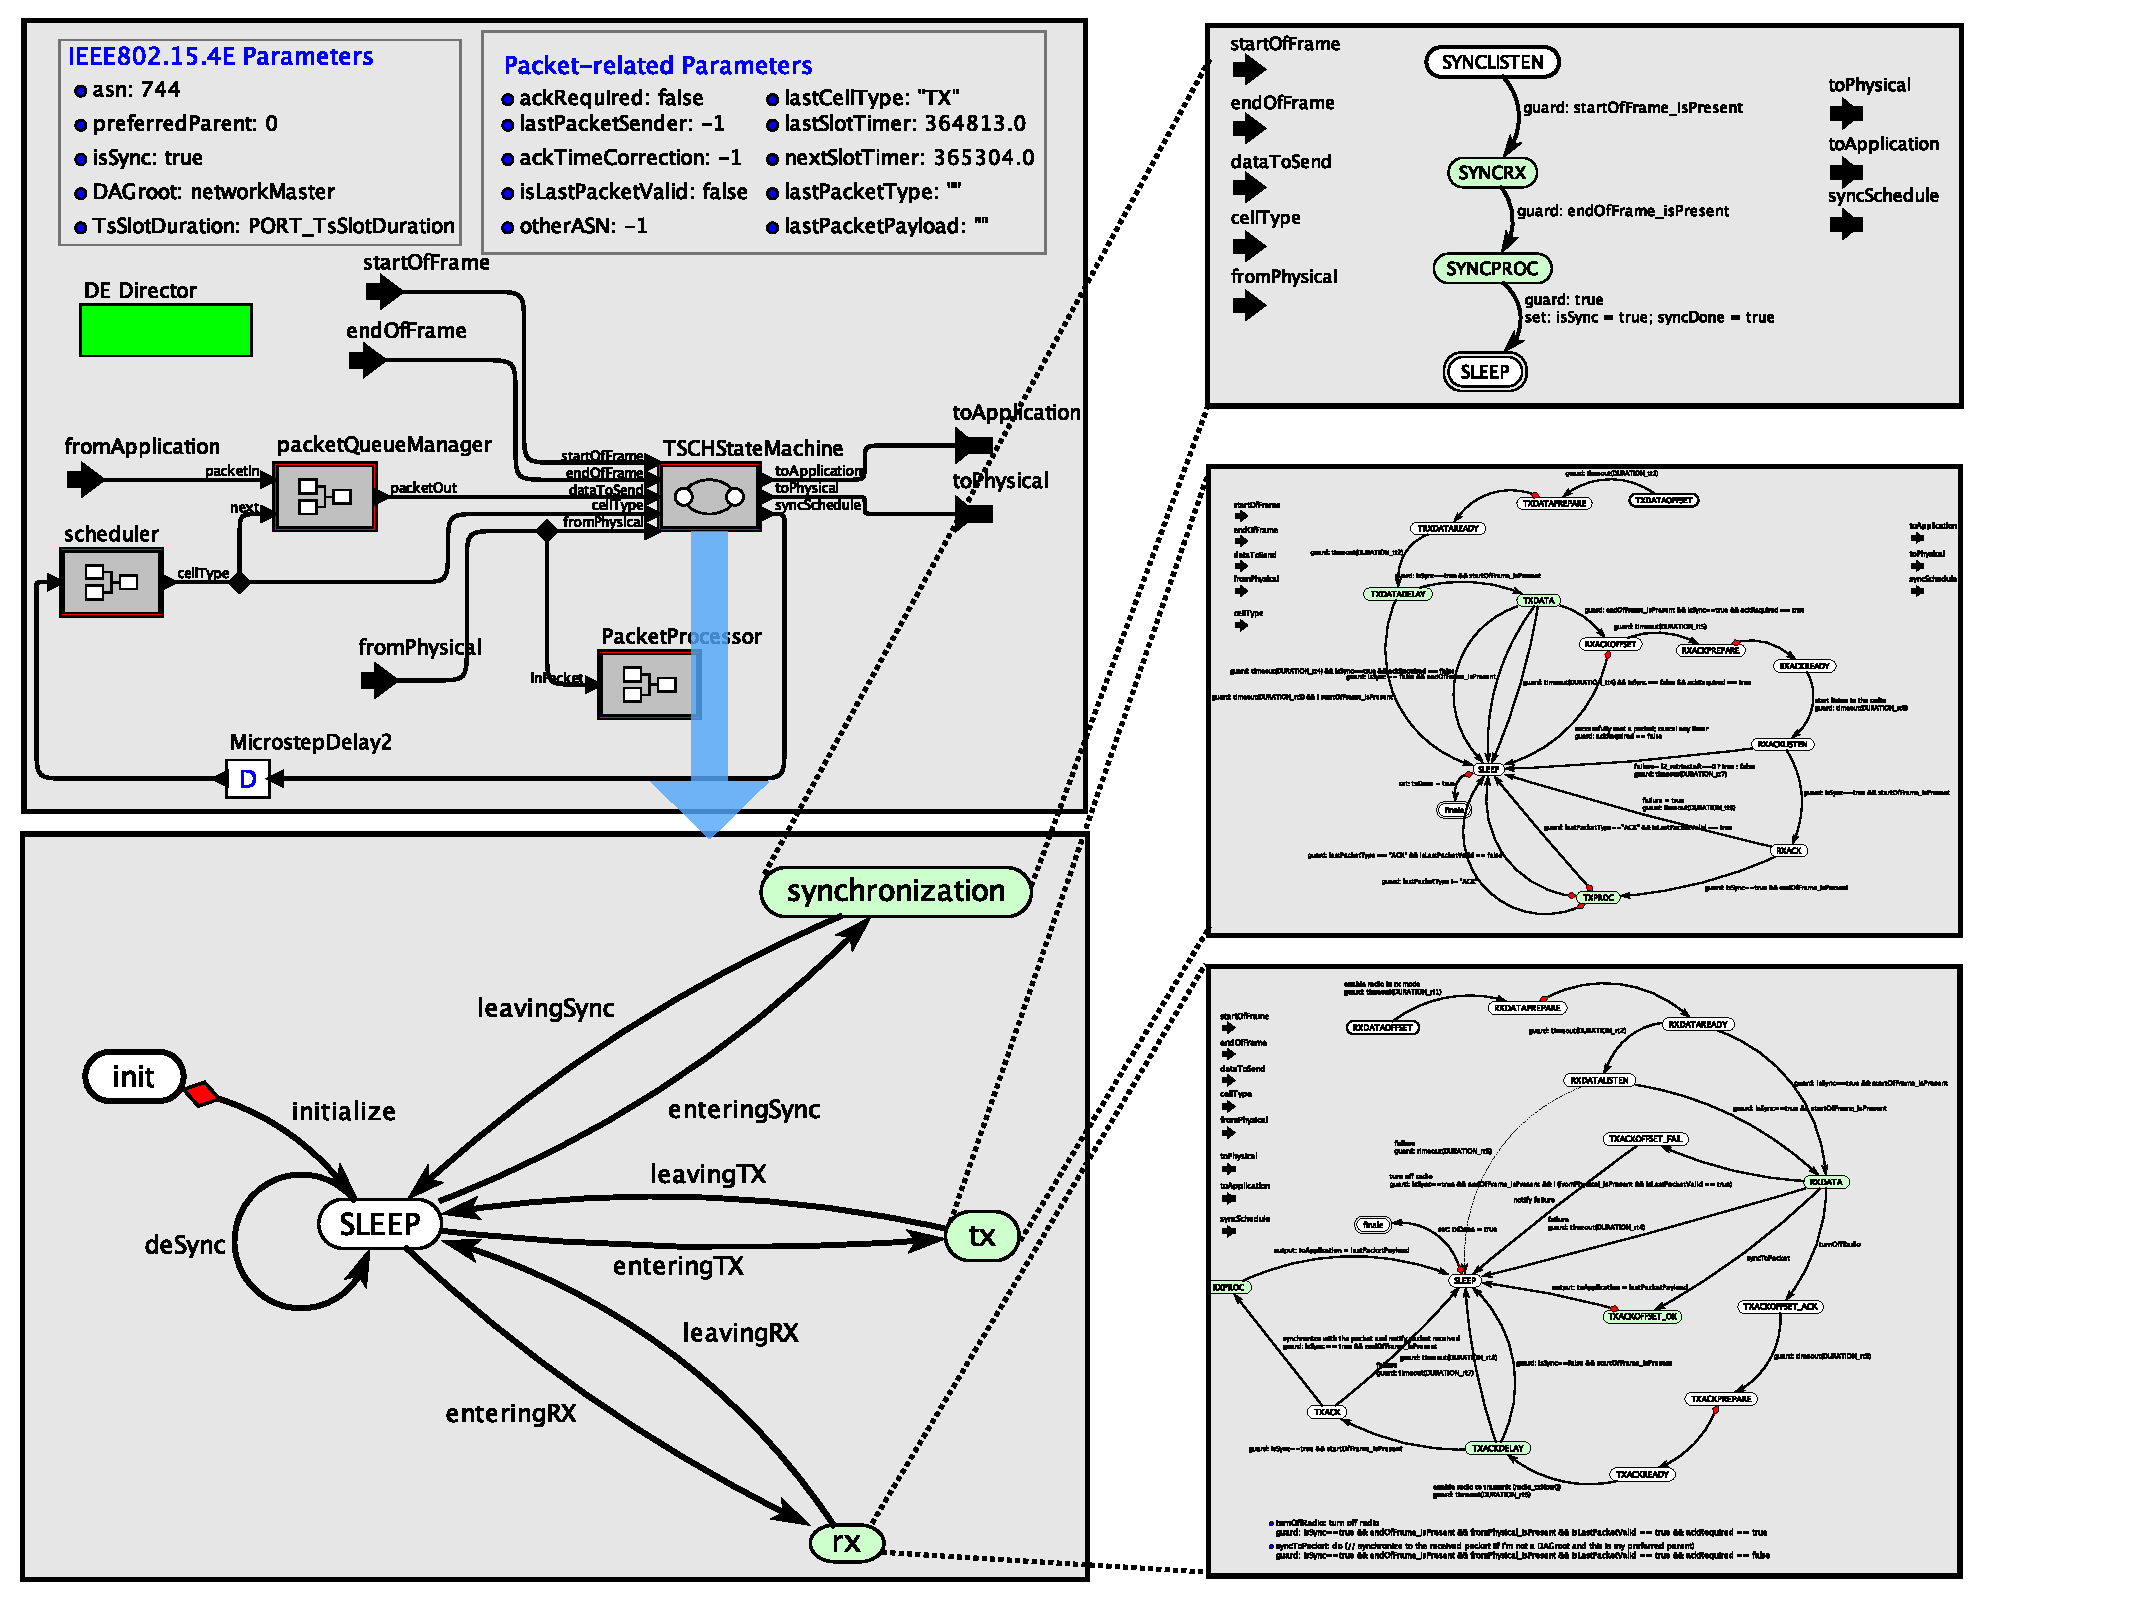
\includegraphics[width=\columnwidth]{figures/PaperTSCHStateMachine}
\caption{\small The state machine with refinements of TSCH protocol. The two subfigures on the bottom-right, being vector graphics, can be easily be read zooming in or checking the attached Ptolemy model}
\label{fig:TSCHSM}
\end{figure}

{\bf MACLayer:} In our model, this is the most important actor. Figure~\ref{fig:TSCHSM} gives an immediate yet detailed overview of its internal structure.
Actors \texttt{packetQueueManager} and \texttt{PacketProcessor} are used to handle packets coming from the application and physical layers. In the first case, since the application sends packets arbitrarily, we need a \emph{queue manager} actor to store packets till the system is allowed to send them. In the second case, since a packet is received from the physical layer only when the MAC layer is in the reception phase, we just need an actor to extract information as the payload, the sender address, the validity of the packet, etc.
\texttt{scheduler} actor is responsible to communicate to the TSCH state machine what is the current slot ASN and when each slot begins. In our model, according to the actual OpenWSN implementation\footref{note:openWSN}, the schedule is predefined for each node. 

The \texttt{TSCHStateMachine} is implementated as a Ptolemy \emph{modal mode actor} and consists of five main states, which describe the node activity: \texttt{init}, \texttt{SLEEP}, \texttt{synchronization}, \texttt{tx} and \texttt{rx}. 

During the initialization phase, all protocol related parameters are reset. When in the \texttt{synchronization} refinement, the node keeps listening for \texttt{ADV} packet and performs slot synchronization and ASN synchronization. Once the synchronization is done, it goes back to \texttt{SLEEP} state.
The scheduler decides node actions: 
\begin{itemize}
\item If the current slot is an \texttt{ADV} slot, then the node enters the \texttt{tx} state and sends an \texttt{ADV} packet. 
\item If it is a \texttt{TX} or \texttt{RXTX} slot and the node has data to send (there are packets queued at \texttt{packetQueueManager} actor), it will enter \texttt{tx} state and send the data packet. 
\item If it's \texttt{RX} slot, or it's \texttt{RXTX} slot but the application doesn't have data to send, the node will enter \texttt{rx} state and listen for packets.
\end{itemize}

In both \texttt{tx} and \texttt{rx} states, there is a refinement which captures the complicated state transitions defined by the OpenWSN MAC layer specification (see Figure~\ref{fig:TSCHSM} on the right). For example, when the node is sending a packet, the \texttt{TSCH} state machine makes a transition from \texttt{SLEEP} to \texttt{tx} and then the associate refinement is enabled. Once in the refinement, the state machine follows a certain number of steps according to precise time constraints. Some states have additional refinements that are used to perform very specific actions. These states include \texttt{TXDATA}, where a packet is actually sent through the radio, or \texttt{TXPROC}, in which the re-synchronization information is extracted from the received \texttt{ACK} packet (see Figure~\ref{fig:timeCorrection}). Given our space constraints, we refer the reader to our Ptolemy model for more details on state transition behavior.

The \texttt{synchronization} state (in the high level \texttt{TSCH} state machine) is only entered when the node just joined the network or when it is not synchronized to the rest of the network anymore. 

In general, for every received packet (both \texttt{DATA} or \texttt{ACK} packet), the node will always capture the reception time (Figure~\ref{fig:timeCorrection} {\em top}). If the packet is from its time master (the node contacted to join the network), it will calculate the time discrepancy and use it for its own re-synchronization (Figure~\ref{fig:timeCorrection} {\em middle}). If the packet is from a time slave, then the node will still compute the time difference and send the correction through the \texttt{ACK} packet (Figure~\ref{fig:timeCorrection} {\em down}).

\begin{figure}[t]
\centering
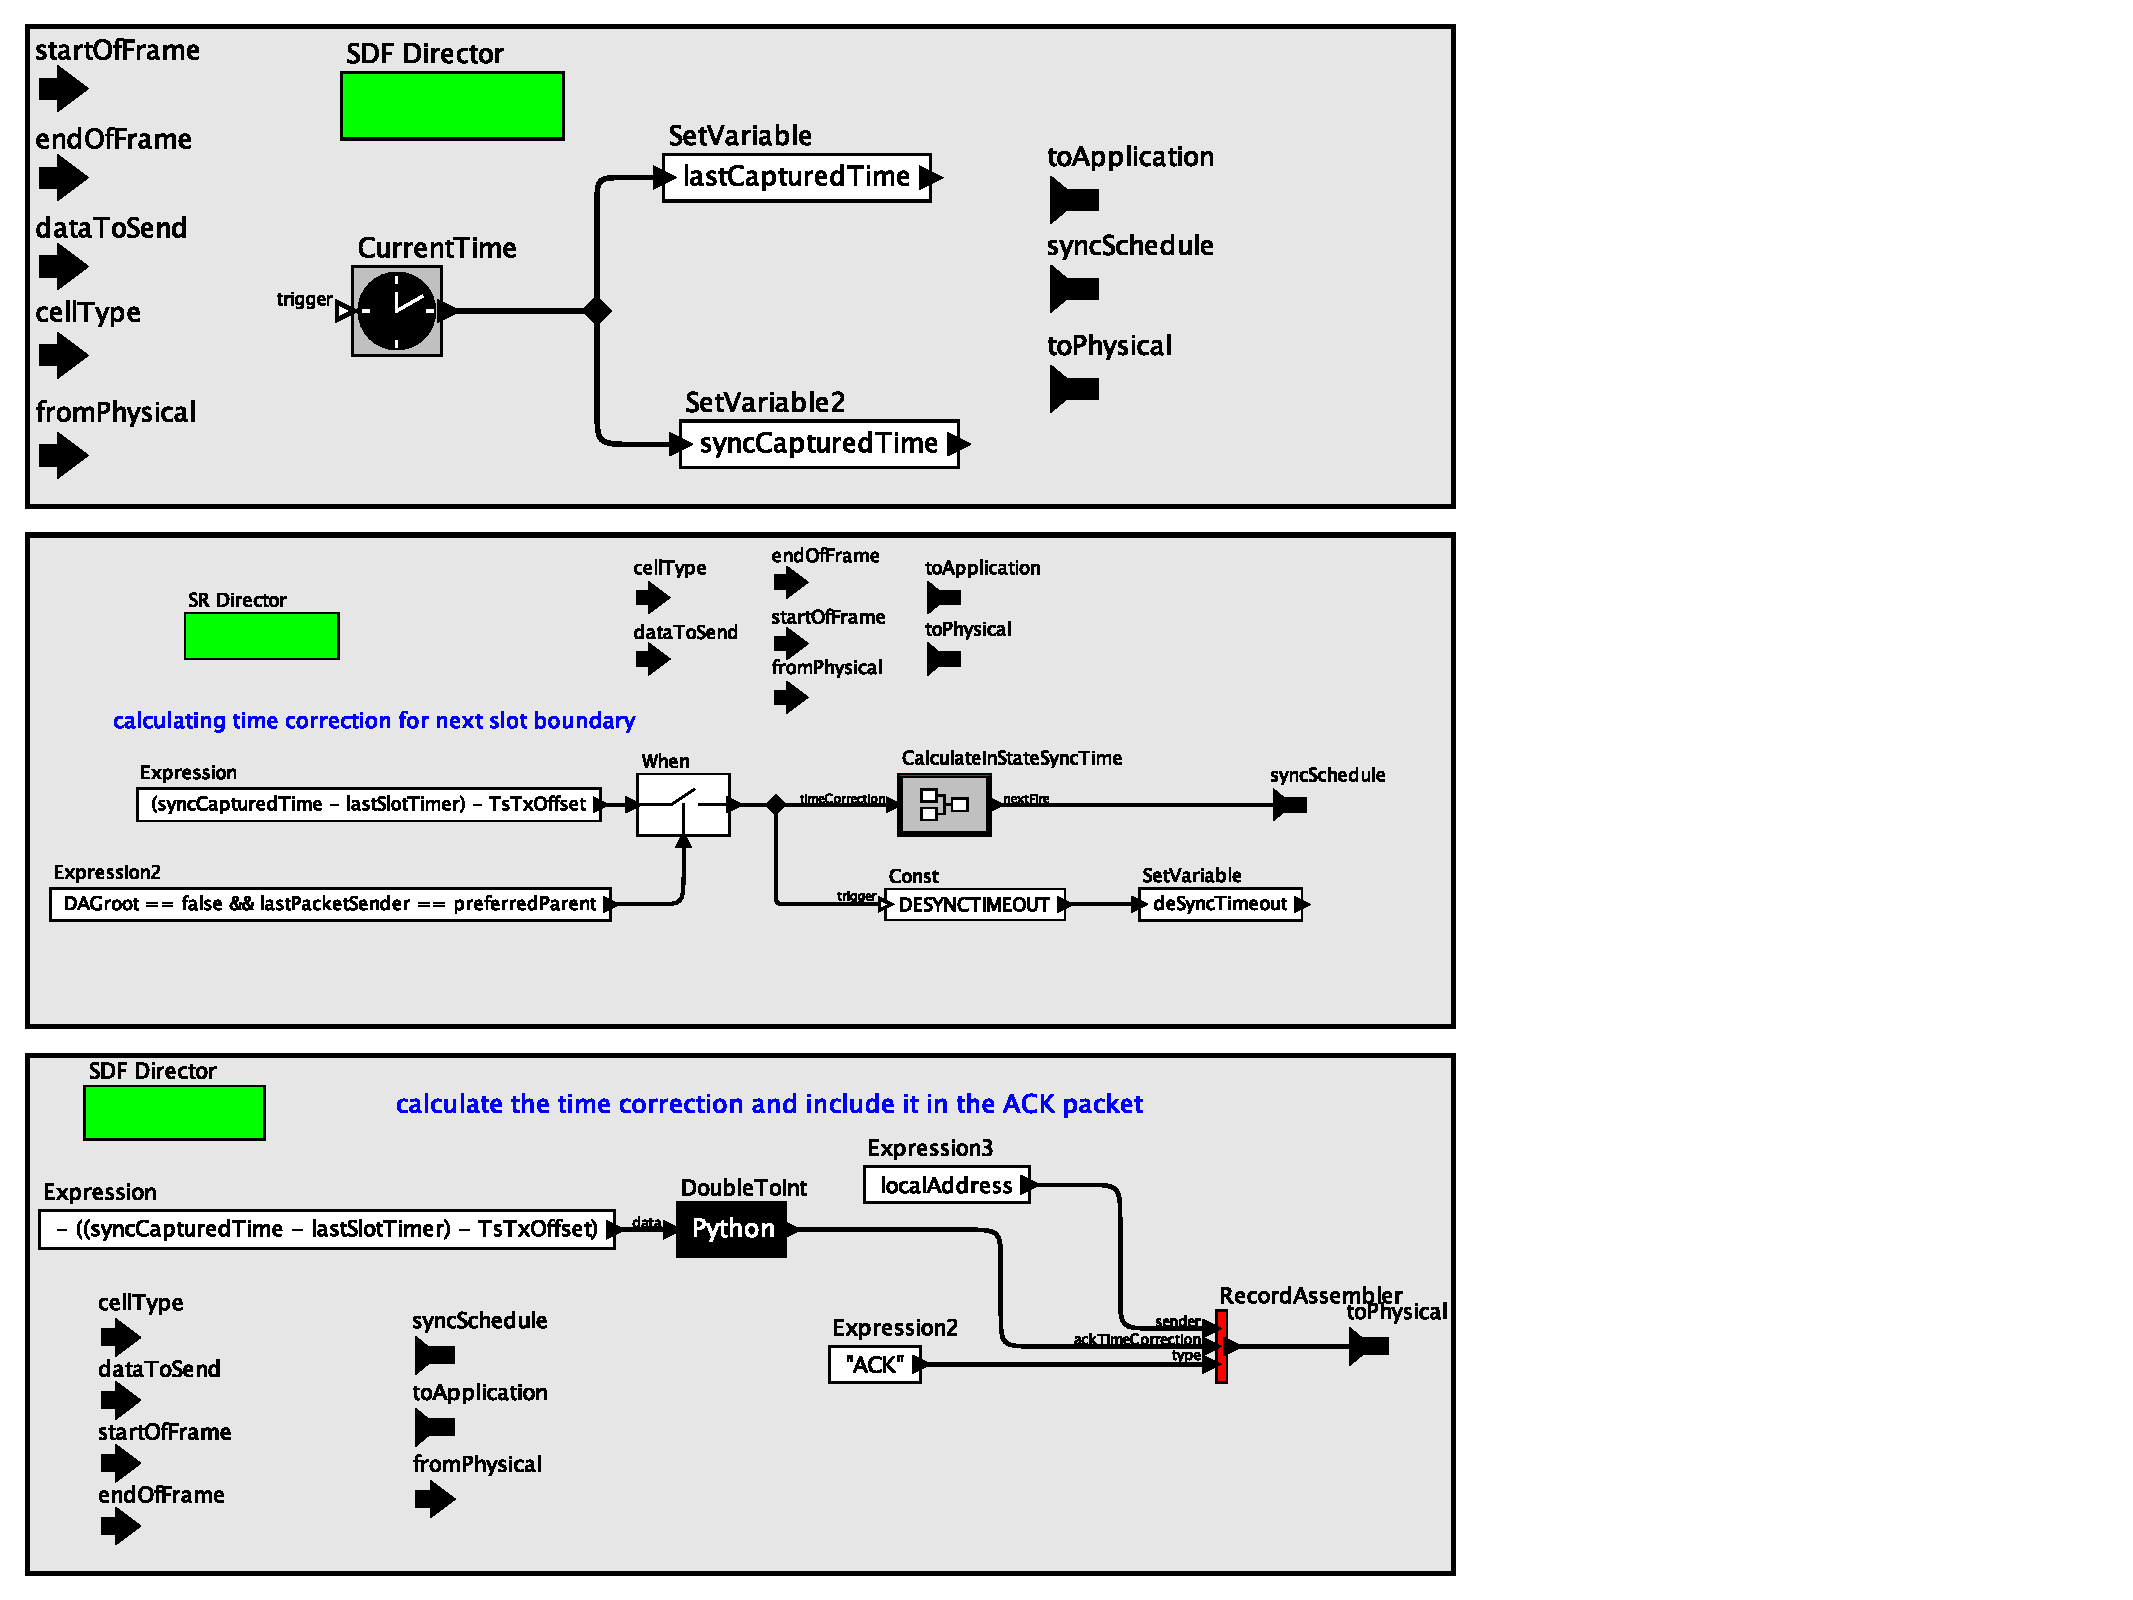
\includegraphics[width=0.8\columnwidth]{figures/PaperReSynchronization}
\caption{\small Modeling the re-synchronization.}
\label{fig:timeCorrection}
\end{figure}


\subsection{Energy Consumption Modeling}
\label{sec:energy}

In \cite{vilajosana2013realistic}, authors measured power consumption values  for several radio chips and microcontrollers running the OpenWSN stack. Moreover, they annotated each state of the OpenWSN \texttt{TSCH} state machine with the correspondent state of the radio and of the microcontroller.
Similarly, we used those radio and microcontroller states to label our \texttt{TSCH} state machine.
For each node, at runtime, an additional actor compute the power consumption value considering the \texttt{TSCH} state machine annotations and the amount of time the MAC layer spends in each state.
For additional details, we suggest to the reader to check the attached model and demos.



%%% Local Variables: 
%%% mode: latex
%%% TeX-master: "ee219d"
%%% End: 
